\chapter{Theory of Equations}
An equation of the form $ax^2 + bx + c = 0$, where $a, b, c\in \mathbb{C}$, the set of complex numbers, is called a \textit{quadratic
  equation}. The numbers $a, b, c$ are called \textit{coefficients} of the equation. The quantity $b^2 - 4ac$ is called the
\textit{discriminant} of the equation. It is represented by $D$ or $\Delta$. A quadratic equation represents a parabola
geometrically.

\noindent\textbf{Examples:}
\begin{enumerate}
\item $4x^2 + 4x + 1 = 0, a = 4, b = 4, c = 1$
\item $7x^3 + 10 = 0$ is not a quadratic equation.
\item $3x^2 -2x^{1/2} + 7 = 0$ is not a quadratic equation.
\item $2x^2 - 4 = 0, a = 2, b = 0, c= -4$
\end{enumerate}

The quadratic equation is called \textit{incomplete} if one of the coefficients $b$ or $c$ is zero. Thus, the last example abpve
represents an incomplete quadratic equation.

An expression of the form $ax^2 + bx + c$ is called a \textit{quadratic expression} while other elements are same as a quadratic
equation.

If two expression in $x$ are equal for all values of $x$ then this statement of equality between the two expression is called an
\textit{identity}.

$f(x) = 0$ is said to be an indentity in $x$ if it is satisfied by all values of $x$ in the domain of $f(x)$. Thus, an indentity in
$x$ is satisfied by all values of $x$ while an equation is satisfied for particular values of $x$.

\noindent\textbf{Example:} $(x + 1)^2 = x^2 + 2x + 1$ is an identity in $x$.

Two equations are called \textit{identical equations} if they have same roots.

\noindent\textbf{Example:} $x^2 - 5x + 4 = 0$ and $2x^2 - 10x + 8 = 0$ are indentical equations because both have same roots $1$ and $4$.

\noindent\textbf{Note:}
\begin{enumerate}
\item Two equations in $x$ are indentical if and only if the coefficients of similar power of $x$ in the two equations are
  proportional. Thus, if $ax^2 + bx + c = 0$ and $a_1x^2 + b_1x + c_1 = 0$ are identical equations, then $\frac{a}{a_1} =
  \frac{b}{b_1} = \frac{c}{c_1}$
\item An equation remains unchanged if it is multiplied or divided by non-zero number.
\end{enumerate}

An expression of the form $a_0x^n + a_1x^{n - 1} + a_2x^{n - 2} + \ldots + a_{n - 1}x + a_0$, where $a_0, a_1, a_2, \ldots, a_n$
are constants $(a_0 \neq 0)$ and $n$ is a positive integer is called a polynomial in $x$ of degree $n$.

As a special case a constant is also called a polynomial of degree zero.

\section{Rational Expression or Rational Function}
An expression of the form $\frac{P(x)}{Q(x)}$, where $P(x)$ and $Q(x)$ are polynomials in $x$, is called a rational expression.

In the particular case, when $Q(x)$ is a non-zero constant, $\frac{P(x)}{Q(x)}$ reduces to a polynomial.Thus, every polynomial is a
rational expression but the converse is not true.

\noindent\textbf{Examples:}
\begin{enumerate}
\item $\frac{x^ - 5x + 4}{x - 2}$
\item $\frac{1}{x - 7}$
\end{enumerate}

\section{Roots of a Quadratic Equation}
The values $x$ for which the equation $ax^2 + bx + c = 0$ are satisfied are called roots of the equation. They are also called
roots of the quadratic expression $ax^2 + bx + c$

Every quadratic equation has at most two roots. Let $ax^2 + bx + c = 0$, where $a\neq 0$

Multiplying both sides of the equation with $a$

$a^2x^2 + abx + ac = 0 \Rightarrow (ax)^2 + 2.ax.\frac{b}{2} + \frac{b^2}{4} + ac - \frac{b^2}{4} = 0$

$\left(ax + \frac{b}{2}\right)^2 = \frac{b^2 - 4ac}{4} \Rightarrow x = \frac{-b \pm\sqrt{b^2 - 4ac}}{2a}$

These are two roots of the quadratic equation. Let us suppose the above quadratic equation has three roots $\alpha, \beta$ and
$\gamma$. These roots will satisfy the above equation. Thus,
$$a\alpha^2 + b\alpha + c = 0, a\beta^2 + b\beta + c = 0, a\gamma^2 + b\gamma + c = 0$$

Subtracting the first two, we get $(\alpha - \beta)[a(\alpha + \beta) + b] = 0$

$\because \alpha \neq \beta \therefore a(\alpha + \beta) + b = 0$

Similarly, $a(\alpha + \gamma) + b = 0$

Subtracting these two, we get $a(\alpha - \gamma) = 0$

$\because a\neq 0 \therefore \alpha = \gamma$

Thus, a quadratic equation has at most two roots.

\section{Sum and Product of the Roots}
From the two obtained  we observe that $\alpha + \beta = -\frac{b}{a}$ and $\alpha\beta = \frac{c}{a}$

\section{Quadratic Expression and its Graph}
Let $f(x) = ax^2 + bx + c$, where $a, b, c\in\mathbb{R}$ and $a\neq 0$.

\begin{equation}
  \label{eq:1}
  f(x) = a\left[\left(x + \frac{b}{2a}\right)^2 + \frac{4ac - b^2}{4a^2}\right]
\end{equation}

\subsection{When a Quadratic Equation is Always Positive/Negative}
It follows from eq. \ref{eq:1}, that $f(x) > 0(< 0)~\forall~x\in\mathbb{R}$ if and only if $a > 0(< 0)$ and $D = b^2 - 4ac <
0$. See Fig. \ref{fig:1}(Fig. \ref{fig:2}). Also, it follows from \ref{eq:1} that $f(x) \geq 0(\leq 0)~\forall~x\in\mathbb{R}$ if
and only if $a > 0(< 0)$ and $D = b^2 - 4ac = 0$. in this case $f(x) < 0(< 0)$ for each $x\in R, x\neq -b/2a$, and the graph of $y
= f(x)$ touches the $x$-axis at $x = -b/2a$.

\begin{figure}[H]
  \begin{center}
    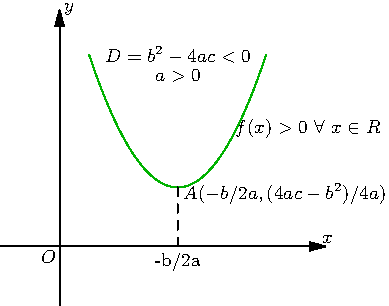
\includegraphics{quadratic-equation-1}
    \caption{When quadratic equation is always positive}
    \label{fig:1}
  \end{center}
\end{figure}

\begin{figure}[H]
  \begin{center}
    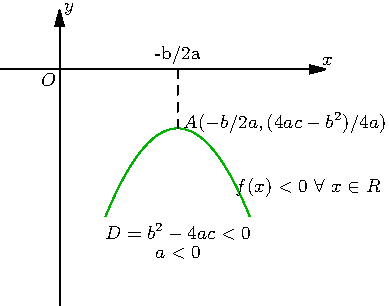
\includegraphics{quadratic-equation-2}
    \caption{When quadratic equation is always negative}
    \label{fig:2}
  \end{center}
\end{figure}

\section{Sign of a Quadratic Equation}
If $D = b^2 - 4ac > 0$, then eq. \ref{eq:1} can be written as

$$f(x) = a\left[\left(x + \frac{b}{2a}\right)^2 - \left(\frac{\sqrt{b^2 - 4ac}}{2a}\right)^2\right]$$
$$= a\left[\left(x + \frac{b + \sqrt{b^2 - 4ac}}{2a}\right)\left(x + \frac{b - \sqrt{b^2 - 4ac}}{2a}\right)\right]$$
$$= a(x - \alpha)(x - \beta)$$

If $D = b^2 - 4ac > 0$ and $a > 0$, then (See Fig. \ref{fig:3})

$$f(x) = \begin{cases}> 0\text{~for~}x <\alpha\text{~or~}x
  >\beta\\>0\text{~for~}\alpha<x<\beta\\=0\text{~for~}x=\alpha,\beta\end{cases}$$

\begin{figure}[H]
  \begin{center}
    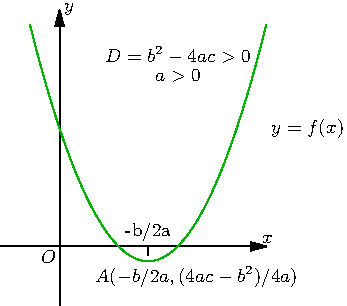
\includegraphics{quadratic-equation-3}
    \caption{When $D > 0$ and $a > 0$}
    \label{fig:3}
  \end{center}
\end{figure}

If $D = b^2 - 4ac > 0$ and $a < 0$, then (See Fig. \ref{fig:4})

$$f(x) = \begin{cases}< 0\text{~for~}x <\alpha\text{~or~}x
  >\beta\\>0\text{~for~}\alpha<x<\beta\\=0\text{~for~}x=\alpha,\beta\end{cases}$$

Note that if $a > 0$, then $f(x)$ attains the least value at $x = -b/2a$, a value which is achieved by differentiating the function
once and at this point the tangent to parabola has slope $0$. The least value is given by
$$f\left(-\frac{b}{2a}\right) = \frac{4ac - b^2}{4a}$$

If $a < 0$, then $f(x)$ is maximum at value $x = -\frac{b}{2a}$ and value of function has the same formula which is for least value
shown above.

\begin{figure}[H]
  \begin{center}
    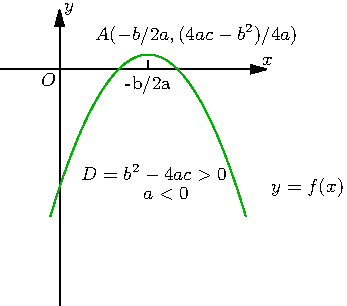
\includegraphics{quadratic-equation-4}
    \caption{When $D > 0$ and $a < 0$}
    \label{fig:4}
  \end{center}
\end{figure}

\section{Position of Roots}
\textbf{Conditions for both roots to be more than a real number $k$}

\begin{figure}[H]
  \begin{center}
    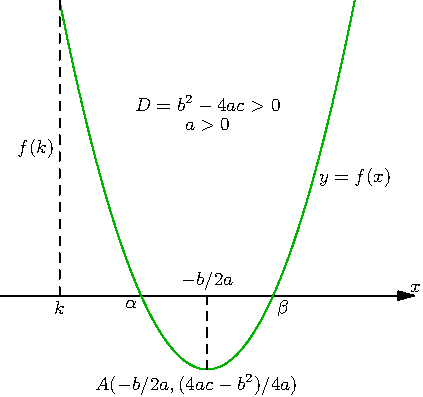
\includegraphics{quadratic-equation-5}
    \caption{When $D > 0$ and $a > 0$}
    \label{fig:5}
  \end{center}
\end{figure}

Form the Fig. \ref{fig:5}, we note that both the roots are more than $k$ if and only if $D>0,~k<-\frac{b}{2a}$ and $f(k)>0$.

In case $a< 0,$ from Fig. \ref{fig:6}, both the roots are more than $k$ if and only if $D>0,~k<-\frac{b}{2a}$ and $f(k)<0$.

\begin{figure}[H]
  \begin{center}
    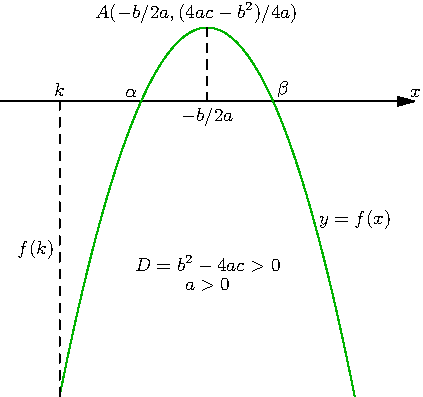
\includegraphics{quadratic-equation-6}
    \caption{When $D > 0$ and $a < 0$}
    \label{fig:6}
  \end{center}
\end{figure}

Combining the above two equations, we get the condition for the roots to be more than a real number $k$ if and only if
$D>0,~k<-\frac{b}{2a}$ and $af(k)>0$. Similarly, condition for the roots to be more than a real number $k$ if and only if
$D>0,~k>-\frac{b}{2a}$ and $af(k)>0$.

\noindent\textbf{Conditions for a real number $k$ to lie between two roots}

Similarly, the real number $k$ lies between the roots of the quadratic equation if and only if $a$ and $f(k)$ are of opposite
signs, i.e. if and only if $a>0,~D>0,~f(k) < 0$ or $a< 0,~D>0,~f(k)>0$.

Combining these two, we get $D>0,~af(k) < 0$ as the condition for $k$ to lie between two roots.

\noindent\textbf{Conditions for exactly one root to lie in between $(k_1, k_2)$ where $k_1<k_2$}

If $a>0$, then exactly one root lies in the interval $(k_1, k_2)$ if and only if $f(k_1)>0$ and $f(k_2)<0$. Also, same is true if
anad only if $f(k_1)<0$ and $f(k_2)>0$. Combining these two we get $f(k_1)f(k_2) < 0$. This condition is also true if $a<0$.

\noindent\textbf{Conditions for both roots to lie in between $(k_1, k_2)$ where $k_1<k_2$}

If $a >0$, both the roots will lies in the interval $(k_1, k_2)$ if and only if $D>0,~k_1<-\frac{b}{2a}<k_2,~f(k_1)>0$ and
$f(k_1)>0$. In case $a<0$, the conditions are $D>0,~k_1<-\frac{b}{2a}<k_2,~f(k_1)<0$ and $f(k_1)<0$.

\noindent\textbf{Conditions for the quadratic equation to have repeated roots}

The quadratic equation $f(x) = ax^2 + bx + c = 0, a\neq 0$ has a repeated root if and only if $f(\alpha) = f'(\alpha) = 0$, where
$\alpha$ is the repeated root. In this case, $f(x) = a(x - \alpha)^2$, In fact, $\alpha = -b/2a$. Geometrically, the $x$-axis will
be a tangent to the parabola at $x = -b/2a$. See Fig. \ref{fig:7} and Fig. \ref{fig:8}.

\begin{figure}[H]
  \begin{center}
    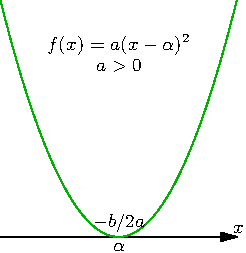
\includegraphics{quadratic-equation-7}
    \caption{$f(\alpha)=0,~f'(\alpha)=0$}
    \label{fig:7}
  \end{center}
\end{figure}

\begin{figure}[H]
  \begin{center}
    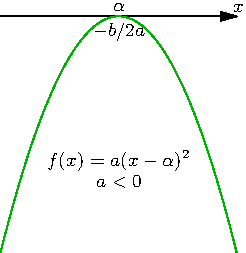
\includegraphics{quadratic-equation-8}
    \caption{$f(\alpha)=0,~f'(\alpha)=0$}
    \label{fig:8}
  \end{center}
\end{figure}

\noindent\textbf{Conditions for two quadratic equations to have one common root}

Consider two quadratic equations $ax^2 + bx + c = 0$ and $a'x^2 + b'x^2 + c' = 0$ having a common root $\alpha$. Clearly, this
common root will satisfy both the equations, i.e. $a\alpha^2 + b\alpha + c = 0$ and $a'\alpha^2 + b'\alpha + c' = 0$.

Solving these two equations, we get

$$\frac{\alpha^2}{bc' - b'c} = \frac{\alpha}{a'c - ac'} = \frac{1}{ab' - a'b}$$
$$\Rightarrow \alpha^2 = \frac{bc' - b'c}{ab' - a'b}, \alpha = \frac{a'c - ac'}{ab' - a'b}$$

Eliminating $\alpha$, we get

$$(a'c - ac')^2 = (bc' - b'c)(ab' - a'b)$$

This is the required condition for two quadratic equations to have one common root.

\begin{figure}[H]
  \begin{center}
    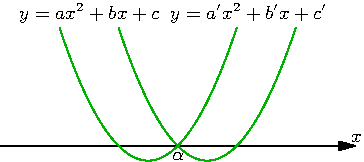
\includegraphics{quadratic-equation-9}
    \caption{Common roots}
    \label{fig:9}
  \end{center}
\end{figure}

\begin{figure}[H]
  \begin{center}
    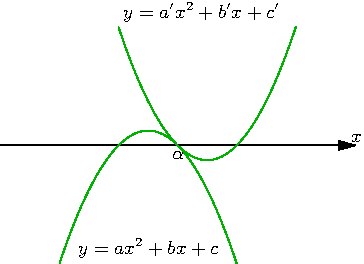
\includegraphics{quadratic-equation-10}
    \caption{Common roots}
    \label{fig:10}
  \end{center}
\end{figure}

To obtain the common root make coefficients of $x^2$ in both the equations same and subtract one equation from the other to obtain
a linear equation in $x$, which you can solve to obtain the common root.

For having both roots common the two equations must be identical i.e. $\frac{a}{a'} = \frac{b}{b'} = \frac{c}{c'}$

\section{General Quadratic Equation in $x$ and $y$}
The general quadratic equation in $x$ and $y$ is given by $ax^2 + 2hxy + by^2 + 2gx + 2fy + c = 0$

$$\therefore x = \frac{-2(hy + g)\pm\sqrt{4(hy + g)^2 - 4a(by^2 + 2fy + c)}}{2a}$$
$$\Rightarrow x + hy + g = \pm \sqrt{(h^2 - ab)y^2 + 2(gh - af)y + g^2 - ac}$$

It can be resolved into two linear factors if $(h^2 - ab)y^2 + 2(gh - af)y + g^2 - ac$ is a perfect square and $h^2 - ab > 0$.

The condition for $(h^2 - ab)y^2 + 2(gh - af)y + g^2 - ac$ to be a perfect square is that its discriminant is $0$, i.e.

$$4(gh - af)^2 - 4(h^2 - ab)(g^2 - ac) = 0$$
$$\Rightarrow abc + 2fgh - af^2 - bg^2 - ch^2 = 0$$
